\chapter{Definitions}
\section{Linear Functions}
One of the most important functions in mathematics is the linear function. A linear function is a function that can be written in the form $f(x) = mx + b$, where $m$ is the slope of the line and $b$ is the $y$-intercept.

\section{Unit Circle}
The unit circle is a circle with a radius of 1. It is centered at the origin of the coordinate plane and is used to define the trigonometric functions.

% Credit for unit circle figure: Supreme Aryal. (2010). Example: Unit circle. \textit{TeXample.net}.  https://texample.net/tikz/examples/unit-circle/ Rights: Licensed under CC BY 2.5 https://creativecommons.org/licenses/by/2.5/ 

\begin{center} 
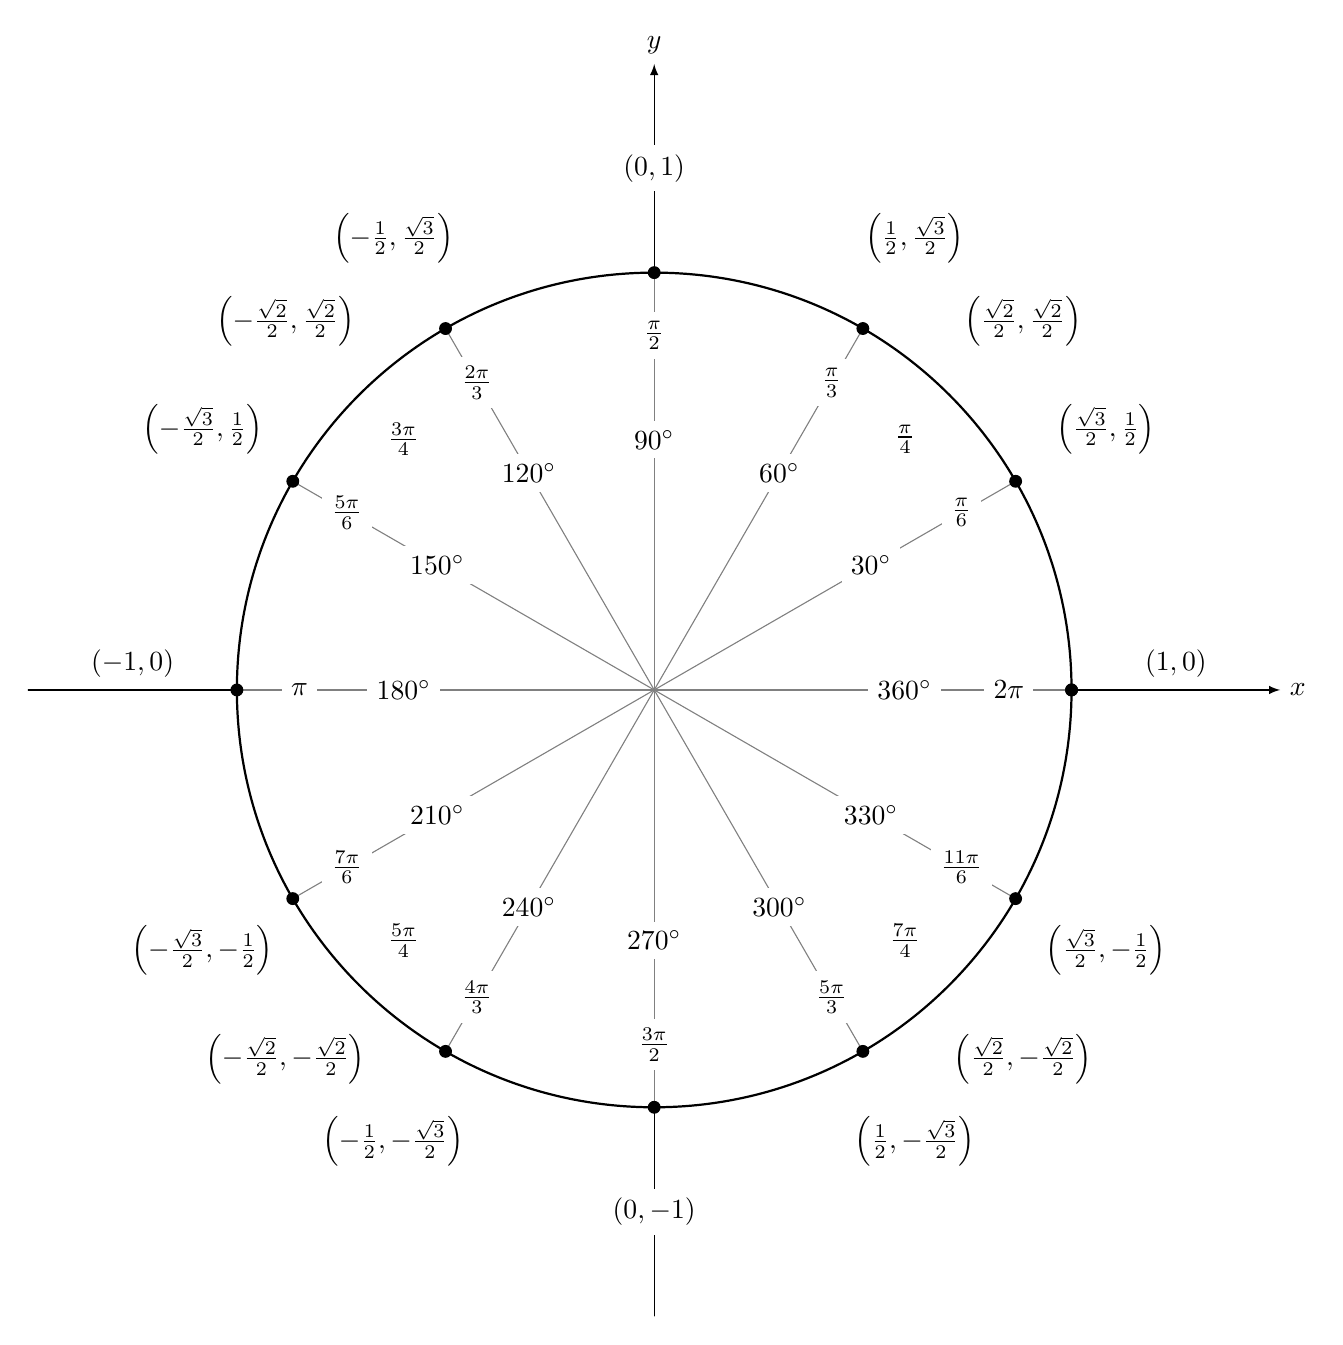
\begin{tikzpicture}[scale=5.3,cap=round,>=latex]
	% draw the coordinates
	\draw[->] (-1.5cm,0cm) -- (1.5cm,0cm) node[right,fill=white] {$x$};
	\draw[->] (0cm,-1.5cm) -- (0cm,1.5cm) node[above,fill=white] {$y$};

	% draw the unit circle
	\draw[thick] (0cm,0cm) circle(1cm);

	\foreach \x in {0,30,...,360} {
			% lines from center to point
			\draw[gray] (0cm,0cm) -- (\x:1cm);
			% dots at each point
			\filldraw[black] (\x:1cm) circle(0.4pt);
			% draw each angle in degrees
			\draw (\x:0.6cm) node[fill=white] {$\x^\circ$};
	}

	% draw each angle in radians
	\foreach \x/\xtext in {
		30/\frac{\pi}{6},
		45/\frac{\pi}{4},
		60/\frac{\pi}{3},
		90/\frac{\pi}{2},
		120/\frac{2\pi}{3},
		135/\frac{3\pi}{4},
		150/\frac{5\pi}{6},
		180/\pi,
		210/\frac{7\pi}{6},
		225/\frac{5\pi}{4},
		240/\frac{4\pi}{3},
		270/\frac{3\pi}{2},
		300/\frac{5\pi}{3},
		315/\frac{7\pi}{4},
		330/\frac{11\pi}{6},
		360/2\pi}
			\draw (\x:0.85cm) node[fill=white] {$\xtext$};

	\foreach \x/\xtext/\y in {
		% the coordinates for the first quadrant
		30/\frac{\sqrt{3}}{2}/\frac{1}{2},
		45/\frac{\sqrt{2}}{2}/\frac{\sqrt{2}}{2},
		60/\frac{1}{2}/\frac{\sqrt{3}}{2},
		% the coordinates for the second quadrant
		150/-\frac{\sqrt{3}}{2}/\frac{1}{2},
		135/-\frac{\sqrt{2}}{2}/\frac{\sqrt{2}}{2},
		120/-\frac{1}{2}/\frac{\sqrt{3}}{2},
		% the coordinates for the third quadrant
		210/-\frac{\sqrt{3}}{2}/-\frac{1}{2},
		225/-\frac{\sqrt{2}}{2}/-\frac{\sqrt{2}}{2},
		240/-\frac{1}{2}/-\frac{\sqrt{3}}{2},
		% the coordinates for the fourth quadrant
		330/\frac{\sqrt{3}}{2}/-\frac{1}{2},
		315/\frac{\sqrt{2}}{2}/-\frac{\sqrt{2}}{2},
		300/\frac{1}{2}/-\frac{\sqrt{3}}{2}}
			\draw (\x:1.25cm) node[fill=white] {$\left(\xtext,\y\right)$};

	% draw the horizontal and vertical coordinates
	% the placement is better this way
	\draw (-1.25cm,0cm) node[above=1pt] {$(-1,0)$}
		  (1.25cm,0cm)  node[above=1pt] {$(1,0)$}
		  (0cm,-1.25cm) node[fill=white] {$(0,-1)$}
		  (0cm,1.25cm)  node[fill=white] {$(0,1)$};
\end{tikzpicture}
\end{center}

Credit: Supreme Aryal \cite{unit} \\ 
Rights: CC BY 2.5

\newpage

\section{Transformations of Functions}

\rowcolors{3}{gray!10}{white!50}
\begin{tabular}{*5l} \toprule
	Transformation of \(f(c>0)\) & Effect on the graph of \(f\) \\ \midrule
   \(f(x)+c\) & Vertical shift up \(c\) units \\
    \(f(x)-c\) & Vertical shift down \(c\) units \\
    \(f(x+c)\) & Shift left by \(c\) units \\
    \(f(x-c)\) & Shift right by \(c\) units \\
	\(cf(x)\) & Vertical Stretch if \(c>1\); vertical compression if \(0<c<1\) \\
	\(f(cx)\) & Horizontal stretch if \(0<c<1\); horizontal compression if \(c>1\) \\
	\(-f(x)\) & Reflection about the \(x\)-axis \\
	\(f(-x)\) & Reflection about the \(y\)-axis \\ \bottomrule
\end{tabular}

	Table 1.7 Transformations of Functions

	\section{Common Angles}

	\rowcolors{3}{gray!10}{white!50}
	\begin{tabular}{*5l} \toprule
		Degrees & Radians & Degrees & Radians \\ \midrule
	   \(0\) & \(0\) & \(120\) & \(\frac{2\pi}{3}\) \\
	\(30\) & \(\frac{\pi}{6}\) & \(135\) & \(\frac{3\pi}{4}\) \\
	\(45\) & \(\frac{\pi}{4}\) & \(150\) & \(\frac{5\pi}{6}\) \\
	\(60\) & \(\frac{\pi}{3}\) & \(180\) & \(\pi\) \\
	\(90\) & \(\frac{\pi}{2}\) & ... & ... \\ \bottomrule
	\end{tabular}

	Table 1.8 Common Angles Expressed in Degrees and Radians

\section{Trigonometric Functions}

	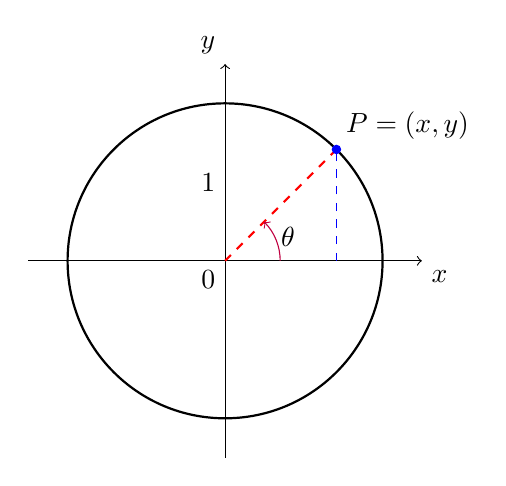
\begin{tikzpicture}
		% Draw the circle
		\draw[thick] (0,0) circle(2cm);
	
		% Draw the x and y axes
		\draw[->] (-2.5, 0) -- (2.5, 0) node[anchor=north west] {$x$};
		\draw[->] (0, -2.5) -- (0, 2.5) node[anchor=south east] {$y$};
	
		% Label 1 on the y-axis
		\node[anchor=east] at (0,1) {$1$};
	
		% Draw the radius line to point P
		\draw[red, thick, dashed] (0,0) -- (45:2);
	
		% Draw the vertical line from x-axis to point P
		\draw[blue, dashed] ({2*cos(45)}, 0) -- ({2*cos(45)}, {2*sin(45)});
	
		% Mark the point P
		\filldraw[blue] (45:2) circle(1.5pt);
		\node[anchor=south west] at (45:2) {$P = (x, y)$};
	
		% Label the origin
		\node[anchor=north east] at (0,0) {$0$};
	
		% Draw the angle theta
		\draw[purple, ->] (0.7,0) arc[start angle=0, end angle=45, radius=0.7cm];
		\node at (0.8, 0.3) {$\theta$};
	
	\end{tikzpicture}

	\textbf{Figure 1.31} The angle \(0\) is in standard position. The values of the trigonometric functions for \(0\) are defined in terms of the coordinates \(x\) and \(y\).

	\newpage 
Let \(P=(x,y)\) be a point on the unit circle centered at the origin \(O\). Let \(\theta\) be an angle with an initial side along the positive \(x\)-axis and a terminal side given by the segment \(OP\). The \textbf{trigonometric functions} are then defined as 

\[\sin\theta=y\]
\[\cos\theta=x\]
\[\tan\theta=\frac{y}{x}\]
\[\csc\theta=\frac{1}{y}\]
\[\sec\theta=\frac{1}{x}\]
\[\cot\theta=\frac{x}{y}\]

If \(x=0\), \(\sec\theta\), and \(\tan\theta\) are defined. If \(y=0\), then \(\cot\theta\) and \(\csc \theta\) are undefined. 

\subsection{Trigonometric Identities} 
\subsubsection{Reciprocal Identities}

\begin{equation}
	\tan \theta = \frac{\sin\theta}{\cos \theta}
\end{equation}

\begin{equation} 
	\csc \theta = \frac{1}{\sin \theta}
\end{equation}

\begin{equation} 
	\cot \theta = \frac{\cos \theta}{\sin \theta}
\end{equation}

\begin{equation} 
	\sec \theta = \frac{1}{\cos \theta}
\end{equation}

\subsubsection{Pythagorean identities}

\begin{equation}
	\sin^2 \theta + \cos^2 \theta = 1
\end{equation}

\begin{equation}
	1 + \tan^2 \theta + 1 = \sec^2 \theta
\end{equation}

\begin{equation}
	1 + \cot^2 \theta = \csc^2 \theta
\end{equation}

\subsubsection{Addition and subtraction formulas}
\begin{equation} 
	\sin(\alpha \pm \beta) = \sin \alpha \cos \beta \pm \cos \alpha \sin \beta
\end{equation}

\begin{equation} 
	\cos(\alpha \pm \beta) = \cos \alpha \cos \beta \mp \sin \alpha \sin \beta
\end{equation}

\subsubsection{Double-angle formulas}
\begin{equation}
	\sin 2\theta = 2 \sin \theta \cos \theta
\end{equation}

\begin{equation} 
	\cos (2\theta) = 2\cos^2 \theta -1 =1-2\sin^2 \theta = \cos ^2 \theta - \sin^2 \theta
\end{equation}